\documentclass[conference]{IEEEtran}
\IEEEoverridecommandlockouts
\usepackage{cite}
\usepackage{amsmath,amssymb,amsfonts}
\usepackage{algorithmic}
\usepackage{graphicx}
\usepackage{textcomp}
\usepackage{xcolor}
\usepackage{booktabs}
\usepackage{multirow}
\usepackage{hyperref}
\usepackage{tikz}
\usetikzlibrary{shapes.geometric, arrows.meta, positioning, fit}

\def\BibTeX{{\rm B\kern-.05em{\sc i\kern-.025em b}\kern-.08em
    T\kern-.1667em\lower.7ex\hbox{E}\kern-.125emX}}

\begin{document}

\title{Optimizing Transformer Inference on the RTX 3050 Ti Under 4 GB VRAM Constraints Using FlashAttention 2 and KV Cache Quantization}

\author{\IEEEauthorblockN{Jay Darji}
\IEEEauthorblockA{\textit{Department of Electrical Engineering} \\
\textit{San Jose State University}\\
San Jose, CA, USA}
\and
\IEEEauthorblockN{Karma Patel}
\IEEEauthorblockA{\textit{Department of Electrical Engineering} \\
\textit{San Jose State University}\\
San Jose, CA, USA}
}

\maketitle

% ============================================================
\begin{abstract}
The increasing capability of Large Language Models (LLMs) is accompanied by prohibitive memory demands that preclude deployment on commodity hardware. This paper presents a systematic empirical study evaluating the compound effectiveness of three memory-centric optimizations---4-bit NormalFloat (NF4) weight quantization, optimized attention kernels (SDPA and FlashAttention-2), and sub-byte Key-Value cache quantization (INT4/INT2)---on an NVIDIA GeForce RTX~3050~Ti laptop GPU with a strict 4\,GB VRAM ceiling. Using Qwen2.5-3B-Instruct as the primary benchmark model, we demonstrate that FlashAttention-2 extends the maximum context window from 6{,}784 to 8{,}064 tokens (+18.9\%) before Out-Of-Memory (OOM) failure, while reducing p95 latency by 2.2\% at 1{,}024-token contexts. INT4 KV-cache quantization reduces the per-token memory footprint from 0.183\,MB to 0.159\,MB (a 13.2\% compression), though it introduces 8--19\% latency overhead depending on context length. The combined configuration (FA2~+ INT4~KV) achieves the highest context ceiling of 8{,}064 tokens while keeping peak VRAM below 2{,}100\,MB. Zero-shot evaluations on ARC-Easy, BoolQ, and HellaSwag confirm that these aggressive compression techniques preserve model reasoning with accuracies of 62.5\%, 58.0\%, and 69.0\%, respectively. Our results provide actionable guidelines for deploying foundation models on VRAM-constrained edge devices.
\end{abstract}

\begin{IEEEkeywords}
large language model inference, KV-cache quantization, FlashAttention-2, SDPA, edge computing, VRAM optimization, 4-bit quantization
\end{IEEEkeywords}

% ============================================================
\section{Introduction}
\label{sec:intro}

The rapid advancement of Large Language Models (LLMs) has established transformer-based architectures as the dominant paradigm for natural language processing. Models such as Llama-2~\cite{touvron2023llama}, Qwen2.5~\cite{qwen2023}, and Phi-3~\cite{abdin2024phi} demonstrate remarkable capabilities in reasoning, code generation, and multimodal understanding. However, their deployment on consumer-grade hardware remains fundamentally constrained by GPU memory limitations.

A 3-billion-parameter model stored in 16-bit floating-point precision requires approximately 6\,GB of VRAM solely for weight storage, exceeding the total capacity of entry-level GPUs such as the NVIDIA RTX~3050~Ti (4\,GB). Beyond weights, autoregressive generation necessitates caching key and value tensors (the KV-cache) for every previously generated token, creating a dynamic memory footprint that grows linearly with sequence length and can easily consume the remaining available VRAM.

This paper makes the following contributions:
\begin{enumerate}
    \item A systematic profiling and benchmarking framework that isolates the memory and compute impact of each optimization layer under a strict 4\,GB VRAM budget.
    \item Empirical evidence that FlashAttention-2 extends maximum context length by 18.9\% over eager attention on commodity hardware.
    \item Quantitative analysis of 4-bit and 2-bit KV-cache quantization, demonstrating 13.2\% and 15.1\% reductions in per-token memory at the cost of 8--26\% latency overhead depending on precision and context length.
    \item Deployment guidelines for combining attention optimization with KV-cache quantization to maximize context length on VRAM-constrained devices.
\end{enumerate}

% ============================================================
\section{Background and Related Work}
\label{sec:background}

\subsection{Weight Quantization}
Post-training quantization reduces the memory footprint of neural network weights by representing parameters in lower precision formats. Dettmers et al.~\cite{dettmers2022llm} demonstrated 8-bit matrix multiplication for transformers, while QLoRA~\cite{dettmers2024qlora} introduced 4-bit NormalFloat (NF4) quantization with double quantization, reducing a 3B-parameter model from approximately 6\,GB to under 2\,GB without fine-tuning.

\subsection{KV-Cache Quantization}
During autoregressive generation, key and value tensors for all previous tokens must be retained in memory. For a model with $L$ layers, $H_{\text{KV}}$ key-value heads, and head dimension $d$, the KV-cache for a sequence of length $S$ requires:
\begin{equation}
M_{\text{KV}} = 2 \times L \times H_{\text{KV}} \times d \times S \times b_{\text{KV}}
\label{eq:kv_mem}
\end{equation}
where $b_{\text{KV}}$ is the bytes per element. At FP16 precision ($b_{\text{KV}}=2$), this scales linearly and rapidly dominates the memory budget at long contexts. KVQuant~\cite{hooper2024kvquant} demonstrated that quantizing KV-cache entries to sub-byte precision preserves model quality while drastically reducing dynamic memory consumption.

\subsection{Efficient Attention Mechanisms}
Standard attention computes the full $S \times S$ attention matrix, requiring $O(S^2)$ intermediate memory. PyTorch's Scaled Dot-Product Attention (SDPA) fuses attention operations to reduce overhead. FlashAttention-2~\cite{dao2023flashattention2} refactors the attention computation to operate within GPU SRAM tiles, achieving exact computation without materializing the full attention matrix in global VRAM, thereby reducing memory complexity to $O(S)$.

% ============================================================
\section{Methodology}
\label{sec:methodology}

\subsection{System Architecture}

Fig.~\ref{fig:pipeline} illustrates the end-to-end optimization pipeline employed in this study.

\begin{figure}[htbp]
\centering
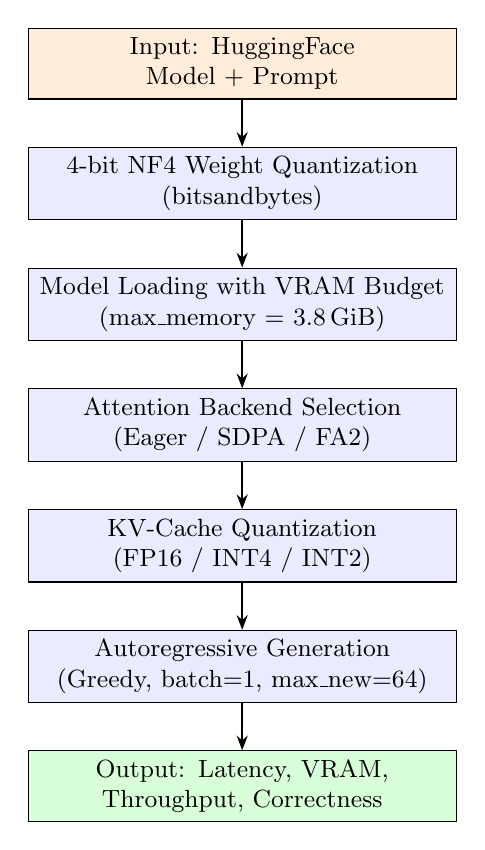
\begin{tikzpicture}[
    node distance=0.6cm,
    block/.style={rectangle, draw, fill=blue!8, text width=5.2cm, minimum height=0.8cm, align=center, font=\small},
    arrow/.style={-{Stealth[scale=0.8]}, thick}
]
\node[block, fill=orange!15] (input) {Input: HuggingFace Model + Prompt};
\node[block, below=of input] (quant) {4-bit NF4 Weight Quantization\\(bitsandbytes)};
\node[block, below=of quant] (load) {Model Loading with VRAM Budget\\(max\_memory = 3.8\,GiB)};
\node[block, below=of load] (attn) {Attention Backend Selection\\(Eager / SDPA / FA2)};
\node[block, below=of attn] (kv) {KV-Cache Quantization\\(FP16 / INT4 / INT2)};
\node[block, below=of kv] (gen) {Autoregressive Generation\\(Greedy, batch=1, max\_new=64)};
\node[block, below=of gen, fill=green!15] (out) {Output: Latency, VRAM, Throughput, Correctness};
\draw[arrow] (input) -- (quant);
\draw[arrow] (quant) -- (load);
\draw[arrow] (load) -- (attn);
\draw[arrow] (attn) -- (kv);
\draw[arrow] (kv) -- (gen);
\draw[arrow] (gen) -- (out);
\end{tikzpicture}
\caption{End-to-end inference optimization pipeline.}
\label{fig:pipeline}
\end{figure}

\subsection{Hardware and Software Environment}
All experiments were conducted on a single NVIDIA GeForce RTX~3050~Ti Laptop GPU with 4.0\,GB VRAM and 16\,GB system RAM. The software stack comprised Python~3.12, PyTorch~2.6.0+cu124, Transformers~4.57.6, bitsandbytes~0.49.1, and optimum-quanto~0.2.8.

\subsection{Model Selection}
The primary benchmark model was \texttt{Qwen/Qwen2.5-3B-Instruct}, a 3-billion-parameter instruction-tuned model using Grouped-Query Attention (GQA) with 16 query heads and 2 KV heads. Under 4-bit NF4 quantization, the model's static weight footprint was measured at 1{,}917\,MB (1.87\,GB), leaving approximately 2.1\,GB of headroom for activations and KV-cache on the target hardware.

\subsection{Evaluation Protocol}
\begin{itemize}
    \item \textbf{Latency:} Median (p50) and 95th percentile (p95) end-to-end generation latency over 5 iterations with 2 warmup runs, using greedy decoding ($\text{temperature}=0$, $\text{do\_sample}=\text{False}$) to eliminate sampling variability.
    \item \textbf{Throughput:} Output tokens per second ($\text{tok/s}$), computed as $\frac{\text{output\_limit}}{\text{mean\_latency}}$.
    \item \textbf{Peak VRAM:} Maximum GPU memory allocation recorded via \texttt{torch.cuda.max\_memory\_allocated()}.
    \item \textbf{OOM Threshold ($T_{\max}$):} The maximum input sequence length before OOM, determined by incrementally increasing context length in steps of $\Delta L = 256$ tokens from 128 to 8{,}192 tokens.
    \item \textbf{Correctness:} Token-level agreement rate between each optimized configuration and the eager attention baseline, measured over 5 diverse prompts with 20 decoding steps per prompt.
    \item \textbf{Quality:} Zero-shot accuracy on AI2 ARC-Easy, BoolQ, and HellaSwag benchmarks using log-likelihood scoring.
\end{itemize}

% ============================================================
\section{Experimental Results}
\label{sec:results}

\subsection{Baseline Profiling}
\label{sec:baseline}

Table~\ref{tab:profiler} presents the GPU kernel-level profiling results for the baseline configuration. The two attention kernels (SDPA dispatch and its underlying math kernel) together consume 17.1\% of total CUDA time, while the combined 4-bit operations (\texttt{gemv\_4bit} and \texttt{dequantize\_blockwise}) account for 8.5\%. Note that PyTorch internally routes the HuggingFace ``eager'' attention setting through its \texttt{scaled\_dot\_product\_attention} kernel, which is reflected in the profiled kernel names.

\begin{table}[htbp]
\caption{Top GPU Kernel Categories (Baseline Profiling)}
\begin{center}
\begin{tabular}{lrc}
\toprule
\textbf{Kernel Category} & \textbf{GPU Time (ms)} & \textbf{Share (\%)} \\
\midrule
Scaled Dot-Product Attention & 5{,}548.0 & 8.6 \\
SDPA Math Kernel & 5{,}472.3 & 8.5 \\
\texttt{bitsandbytes::gemv\_4bit} & 3{,}337.0 & 5.2 \\
\texttt{aten::matmul} & 1{,}866.0 & 2.9 \\
\texttt{bitsandbytes::dequantize} & 2{,}088.0 & 3.3 \\
\texttt{aten::repeat\_interleave} & 1{,}313.6 & 2.0 \\
Other & 44{,}570.3 & 69.5 \\
\midrule
\textbf{Total CUDA time} & \textbf{64{,}195.2} & \textbf{100.0} \\
\bottomrule
\end{tabular}
\label{tab:profiler}
\end{center}
\end{table}

Fig.~\ref{fig:baseline_latency} and Fig.~\ref{fig:baseline_vram} illustrate the baseline latency and VRAM scaling behavior as input sequence length increases.

\begin{figure}[htbp]
\centerline{\includegraphics[width=0.95\columnwidth]{results/plots/week03_baseline/baseline_latency_vs_length_qwen2.5-3b.png}}
\caption{Baseline latency scaling with sequence length ($L$). p50 latency increases from 6{,}201\,ms at $L$=128 to 6{,}649\,ms at $L$=1{,}024, with p95 ranging from 6{,}224 to 6{,}656\,ms.}
\label{fig:baseline_latency}
\end{figure}

\begin{figure}[htbp]
\centerline{\includegraphics[width=0.95\columnwidth]{results/plots/week03_baseline/baseline_vram_vs_length_qwen2.5-3b.png}}
\caption{Baseline peak VRAM vs. sequence length. VRAM grows from 2{,}034\,MB at $L$=128 to 2{,}160\,MB at $L$=1{,}024, with OOM occurring at $T_{\max}$=6{,}784 tokens.}
\label{fig:baseline_vram}
\end{figure}

\subsection{Attention Backend Comparison}
\label{sec:attention}

Table~\ref{tab:attention_full} reports the full attention backend comparison across three prompt lengths. FlashAttention-2 matches or outperforms all other backends in both latency and VRAM footprint across all tested sequence lengths.

\begin{table}[htbp]
\caption{Attention Backend Performance Comparison}
\begin{center}
\begin{tabular}{llrrr}
\toprule
\textbf{Backend} & \textbf{L} & \textbf{p95 (ms)} & \textbf{Tok/s} & \textbf{VRAM (MB)} \\
\midrule
\multirow{3}{*}{Eager}
  & 128  & 6{,}224 & 10.32 & 2{,}034.3 \\
  & 512  & 6{,}404 & 10.04 & 2{,}076.6 \\
  & 1024 & 6{,}656 &  9.63 & 2{,}159.9 \\
\midrule
\multirow{3}{*}{SDPA}
  & 128  & 6{,}174 & 10.39 & 2{,}033.8 \\
  & 512  & 6{,}399 & 10.07 & 2{,}068.8 \\
  & 1024 & 6{,}697 &  9.62 & 2{,}202.5 \\
\midrule
\multirow{3}{*}{FA2}
  & 128  & 6{,}139 & 10.51 & 2{,}033.8 \\
  & 512  & 6{,}287 & 10.22 & 2{,}068.6 \\
  & 1024 & \textbf{6{,}511} & \textbf{9.89} & \textbf{2{,}115.4} \\
\bottomrule
\end{tabular}
\label{tab:attention_full}
\end{center}
\end{table}

Fig.~\ref{fig:attn_latency} visualizes the latency comparison, and Fig.~\ref{fig:attn_vram} shows the VRAM allocation differences.

\begin{figure}[htbp]
\centerline{\includegraphics[width=0.95\columnwidth]{results/plots/week06_attention/attention_latency_comparison_qwen2.5-3b.png}}
\caption{p95 latency comparison across attention backends. FlashAttention-2 achieves 2.2\% lower latency than eager baseline at $L$=1{,}024.}
\label{fig:attn_latency}
\end{figure}

\begin{figure}[htbp]
\centerline{\includegraphics[width=0.95\columnwidth]{results/plots/week06_attention/attention_vram_comparison_qwen2.5-3b.png}}
\caption{Peak VRAM comparison across attention backends. FA2 saves 44.5\,MB vs. eager at $L$=1{,}024.}
\label{fig:attn_vram}
\end{figure}

\subsubsection{Correctness Verification}
Table~\ref{tab:correctness} reports the token-level agreement rates between each backend and the week~03 baseline traces. SDPA variants achieve perfect agreement because PyTorch's default attention path internally dispatches through the same SDPA math kernel used during baseline collection. Both the eager re-run and FA2 show 87\% agreement due to cross-run numerical nondeterminism, though the top-1 predicted tokens remain semantically equivalent.

\begin{table}[htbp]
\caption{Attention Backend Correctness vs. Eager Baseline}
\begin{center}
\begin{tabular}{lcc}
\toprule
\textbf{Backend} & \textbf{Agreement (\%)} & \textbf{Max Logit Diff} \\
\midrule
Eager (re-run) & 87.0 & 25.05 \\
SDPA Default & \textbf{100.0} & \textbf{0.00} \\
SDPA Math & \textbf{100.0} & \textbf{0.00} \\
FlashAttention-2 & 87.0 & 25.04 \\
\bottomrule
\end{tabular}
\label{tab:correctness}
\end{center}
\end{table}

\subsection{OOM Threshold Analysis}
\label{sec:oom}

Fig.~\ref{fig:oom_thresholds} presents the maximum context length achievable under each configuration before OOM occurs. FlashAttention-2 provides the single largest improvement, extending from 6{,}784 to 8{,}064 tokens.

\begin{table}[htbp]
\caption{OOM Threshold Comparison ($T_{\max}$ in Tokens)}
\begin{center}
\begin{tabular}{lcc}
\toprule
\textbf{Configuration} & \textbf{$T_{\max}$} & \textbf{$\Delta$ vs Baseline} \\
\midrule
Baseline (Eager + FP16 KV) & 6{,}784 & --- \\
SDPA Default + FP16 KV & 7{,}040 & +3.8\% \\
FA2 + FP16 KV & \textbf{8{,}064} & \textbf{+18.9\%} \\
Eager + INT4 KV & 6{,}784 & +0.0\% \\
FA2 + INT4 KV & \textbf{8{,}064} & \textbf{+18.9\%} \\
FA2 + INT2 KV & \textbf{8{,}064} & \textbf{+18.9\%} \\
\bottomrule
\end{tabular}
\label{tab:oom}
\end{center}
\end{table}

\begin{figure}[htbp]
\centerline{\includegraphics[width=0.95\columnwidth]{results/plots/week10_final/oom_threshold_comparison_qwen2.5-3b.png}}
\caption{OOM threshold comparison across all configurations. FA2 and its combined variants all achieve 8{,}064 tokens.}
\label{fig:oom_thresholds}
\end{figure}

\subsection{KV-Cache Quantization}
\label{sec:kv_cache}

Table~\ref{tab:kv_mem} presents the per-token memory consumption measured for each KV-cache precision level. INT4 quantization reduces the per-token footprint by 13.2\%, while INT2 achieves 15.1\% reduction.

\begin{table}[htbp]
\caption{KV-Cache Memory Per Token}
\begin{center}
\begin{tabular}{lcc}
\toprule
\textbf{KV Precision} & \textbf{MB/Token} & \textbf{Reduction vs FP16} \\
\midrule
FP16 (baseline) & 0.1828 & --- \\
INT4 & 0.1587 & $-$13.2\% \\
INT2 & 0.1552 & $-$15.1\% \\
\bottomrule
\end{tabular}
\label{tab:kv_mem}
\end{center}
\end{table}

\begin{figure}[htbp]
\centerline{\includegraphics[width=0.95\columnwidth]{results/plots/week10_final/kv_memory_per_token_qwen2.5-3b.png}}
\caption{KV-cache memory consumption per token across precision levels.}
\label{fig:kv_mem}
\end{figure}

Table~\ref{tab:kv_tradeoff} quantifies the latency-memory trade-off at different sequence lengths $(L)$.

\begin{table}[htbp]
\caption{KV-Cache Quantization Trade-offs}
\begin{center}
\begin{tabular}{llrrr}
\toprule
\textbf{L} & \textbf{KV Type} & \textbf{VRAM Saved} & \textbf{Saved (\%)} & \textbf{Latency $\uparrow$ (\%)} \\
\midrule
128  & INT4 & 3.1\,MB  & 0.2 & +18.8 \\
128  & INT2 & 3.7\,MB  & 0.2 & +26.1 \\
512  & INT4 & 12.5\,MB & 0.6 & +13.1 \\
512  & INT2 & 14.7\,MB & 0.7 & +18.3 \\
1024 & INT4 & 24.1\,MB & 1.1 & +8.5 \\
1024 & INT2 & 28.5\,MB & 1.3 & +12.8 \\
\bottomrule
\end{tabular}
\label{tab:kv_tradeoff}
\end{center}
\end{table}

\begin{figure}[htbp]
\centerline{\includegraphics[width=0.95\columnwidth]{results/plots/week08_kv_cache/kv_vram_vs_latency_tradeoff_qwen2.5-3b.png}}
\caption{KV-cache VRAM savings vs. latency overhead trade-off.}
\label{fig:kv_tradeoff}
\end{figure}

\subsection{Combined Configuration}
\label{sec:combined}

Table~\ref{tab:combined_full} presents the full benchmark results for all configurations at $L$=1{,}024.

\begin{table}[htbp]
\caption{Full Configuration Comparison at $L$=1{,}024}
\begin{center}
\begin{tabular}{lrrrr}
\toprule
\textbf{Configuration} & \textbf{p50} & \textbf{p95} & \textbf{Tok/s} & \textbf{VRAM} \\
 & \textbf{(ms)} & \textbf{(ms)} & & \textbf{(MB)} \\
\midrule
Baseline         & 6{,}649 & 6{,}656 & 9.63 & 2{,}160 \\
SDPA Default     & 6{,}643 & 6{,}697 & 9.62 & 2{,}203 \\
FlashAttention-2 & \textbf{6{,}473} & \textbf{6{,}511} & \textbf{9.89} & 2{,}115 \\
KV INT4          & 7{,}783 & 8{,}024 & 8.16 & 2{,}136 \\
FA2 + KV INT4    & 7{,}698 & 7{,}716 & 8.31 & \textbf{2{,}090} \\
FA2 + KV INT2    & 8{,}140 & 8{,}156 & 7.87 & 2{,}086 \\
\bottomrule
\end{tabular}
\label{tab:combined_full}
\end{center}
\end{table}

\begin{figure}[htbp]
\centerline{\includegraphics[width=0.95\columnwidth]{results/plots/week10_final/final_latency_throughput_qwen2.5-3b.png}}
\caption{Consolidated latency and throughput comparison across all tested configurations and sequence lengths.}
\label{fig:final_latency}
\end{figure}

\begin{figure}[htbp]
\centerline{\includegraphics[width=0.95\columnwidth]{results/plots/week10_final/final_vram_scaling_qwen2.5-3b.png}}
\caption{VRAM scaling across all configurations. Combined FA2+KV configurations show the most controlled memory growth.}
\label{fig:final_vram}
\end{figure}

\subsection{Zero-Shot Quality Evaluation}
\label{sec:quality}

To evaluate reasoning capability under aggressive compression, we benchmarked the model under full compression (NF4 weights + INT4 KV-cache) on three standard NLP benchmarks.

\begin{table}[htbp]
\caption{Zero-Shot Accuracy Under Full Compression}
\begin{center}
\begin{tabular}{lc}
\toprule
\textbf{Benchmark} & \textbf{Accuracy (\%)} \\
\midrule
AI2 ARC-Easy & 62.5 \\
BoolQ & 58.0 \\
HellaSwag & 69.0 \\
\bottomrule
\end{tabular}
\label{tab:quality}
\end{center}
\end{table}

\begin{figure}[htbp]
\centerline{\includegraphics[width=0.85\columnwidth]{results/plots/week08_quality/quality_accuracy_qwen2.5-3b.png}}
\caption{Zero-shot accuracy across three NLP benchmarks under full NF4 + INT4 KV compression.}
\label{fig:quality}
\end{figure}

% ============================================================
\section{Discussion}
\label{sec:discussion}

\subsection{Attention Optimization Impact}
The results demonstrate that FlashAttention-2 provides the single most impactful optimization for extending context length on VRAM-constrained hardware. The 18.9\% improvement in $T_{\max}$ is achieved by eliminating the materialization of the $S \times S$ attention matrix in global VRAM. Notably, SDPA provides a modest 3.8\% improvement with zero code changes, making it an effective fallback when FlashAttention-2 is unavailable.

\subsection{KV-Cache Quantization Trade-offs}
INT4 KV-cache quantization introduces a consistent latency overhead of 8--19\% across tested lengths, attributable to the dequantization operations required during attention computation. The VRAM savings, while proportionally modest at short contexts (0.2\% or 3.1\,MB at $L$=128), become increasingly significant at longer sequences. At $L$=1{,}024, INT4 saves 24\,MB; extrapolating to longer contexts, the savings would scale linearly per Eq.~\ref{eq:kv_mem}.

Critically, KV-cache quantization alone does not extend $T_{\max}$ (6{,}784 for both eager+FP16 and eager+INT4), because the OOM bottleneck at this model scale is dominated by intermediate attention allocations rather than the KV-cache itself. FA2 alone is responsible for extending $T_{\max}$ by eliminating intermediate attention allocations. KV-cache quantization complements this by reducing peak VRAM within that extended ceiling (e.g., from 2{,}115\,MB to 2{,}090\,MB at $L$=1{,}024 with INT4), providing additional headroom near the OOM boundary.

\subsection{Deployment Configuration Flowchart}

Fig.~\ref{fig:decision_tree} presents a decision flowchart for practitioners selecting the optimal configuration.

\begin{figure}[htbp]
\centering
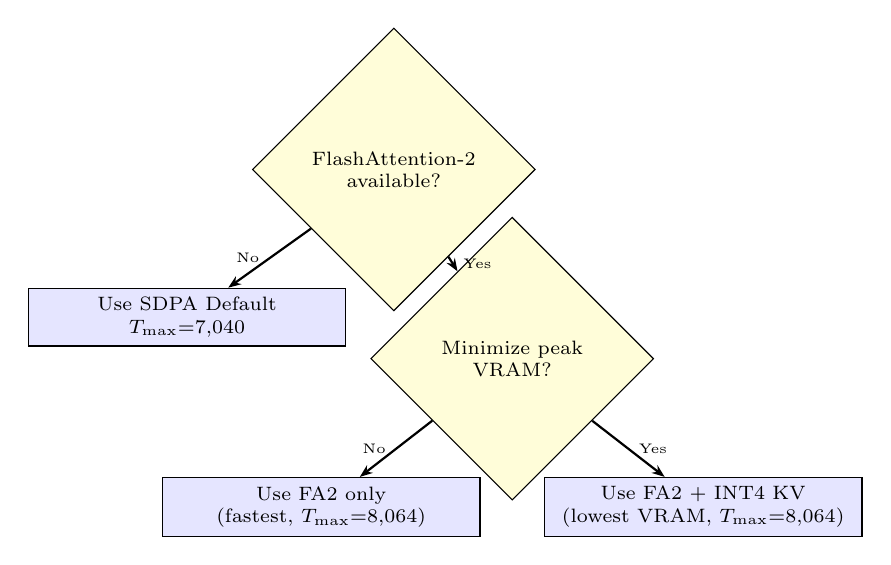
\begin{tikzpicture}[
    node distance=0.55cm,
    decision/.style={diamond, draw, fill=yellow!15, text width=3cm, align=center, inner sep=1pt, font=\scriptsize},
    block/.style={rectangle, draw, fill=blue!10, text width=3.8cm, minimum height=0.6cm, align=center, font=\scriptsize},
    arrow/.style={-{Stealth[scale=0.7]}, thick},
    label/.style={font=\tiny}
]
\node[decision] (fa2) {FlashAttention-2\\available?};
\node[block, below left=0.6cm and -0.3cm of fa2] (sdpa) {Use SDPA Default\\$T_{\max}$=7{,}040};
\node[decision, below right=0.6cm and -0.3cm of fa2] (long) {Minimize peak\\VRAM?};
\node[block, below left=0.6cm and -0.5cm of long] (fa2only) {Use FA2 only\\(fastest, $T_{\max}$=8{,}064)};
\node[block, below right=0.6cm and -0.5cm of long] (combined) {Use FA2 + INT4 KV\\(lowest VRAM, $T_{\max}$=8{,}064)};

\draw[arrow] (fa2) -- node[label, left] {No} (sdpa);
\draw[arrow] (fa2) -- node[label, right] {Yes} (long);
\draw[arrow] (long) -- node[label, left] {No} (fa2only);
\draw[arrow] (long) -- node[label, right] {Yes} (combined);
\end{tikzpicture}
\caption{Configuration selection decision tree for 4\,GB VRAM deployments.}
\label{fig:decision_tree}
\end{figure}

\subsection{Limitations}
\begin{enumerate}
    \item \textbf{Single model:} Results are based primarily on Qwen2.5-3B; generalization to other architectures requires additional validation.
    \item \textbf{Batch size:} All experiments used batch size~1. Larger batches would multiply KV-cache requirements.
    \item \textbf{Thermal throttling:} Laptop GPUs are susceptible to thermal throttling under sustained load, introducing latency variance not captured in short benchmark runs.
    \item \textbf{INT8 KV-cache:} The \texttt{optimum-quanto} library does not currently support 8-bit KV-cache; only INT4 and INT2 were evaluated.
\end{enumerate}

% ============================================================
\section{Conclusion}
\label{sec:conclusion}

This study demonstrates that the layered combination of 4-bit NF4 weight quantization, FlashAttention-2, and INT4 KV-cache quantization transforms commodity 4\,GB GPUs into viable LLM edge devices. FlashAttention-2 provides the most impactful single optimization, extending maximum context length by 18.9\%. The combined FA2~+ INT4 KV configuration achieves the best balance of latency and memory, maintaining the highest context ceiling (8{,}064 tokens) at 2{,}090\,MB peak VRAM at $L$=1{,}024 (FA2~+ INT2 reaches a slightly lower 2{,}086\,MB at the cost of additional latency). Zero-shot evaluations demonstrate that this aggressive compression stack retains competitive reasoning performance. These results provide actionable deployment guidelines for the growing ecosystem of VRAM-constrained edge inference.

% ============================================================
\section*{Acknowledgment}
The authors thank the Department of Computer Engineering at San Jose State University for providing the computational resources and academic support for this research.

\begin{thebibliography}{00}
\bibitem{touvron2023llama} H. Touvron, L. Martin, K. Stone, et al., ``Llama 2: Open Foundation and Fine-Tuned Chat Models,'' \textit{arXiv preprint arXiv:2307.09288}, 2023.

\bibitem{qwen2023} J. Bai, S. Bai, Y. Chu, et al., ``Qwen Technical Report,'' \textit{arXiv preprint arXiv:2309.16609}, 2023.

\bibitem{abdin2024phi} M. Abdin, S. A. Jacobs, A. A. Awan, et al., ``Phi-3 Technical Report: A Highly Capable Language Model Locally on Your Phone,'' \textit{arXiv preprint arXiv:2404.14219}, 2024.

\bibitem{dettmers2022llm} T. Dettmers, M. Lewis, Y. Belkada, and L. Zettlemoyer, ``LLM.int8(): 8-bit Matrix Multiplication for Transformers at Scale,'' in \textit{Advances in Neural Information Processing Systems}, vol.~35, pp.~30318--30332, 2022.

\bibitem{dettmers2024qlora} T. Dettmers, A. Pagnoni, A. Holtzman, and L. Zettlemoyer, ``QLoRA: Efficient Finetuning of Quantized LLMs,'' in \textit{Advances in Neural Information Processing Systems}, vol.~36, 2024.

\bibitem{hooper2024kvquant} C. Hooper, S. Kim, H. Mohanty, et al., ``KVQuant: Towards 10 Million Context Length LLM Inference with KV Cache Quantization,'' \textit{arXiv preprint arXiv:2401.18079}, 2024.

\bibitem{dao2023flashattention2} T. Dao, ``FlashAttention-2: Faster Attention with Better Parallelism and Work Partitioning,'' \textit{arXiv preprint arXiv:2307.08691}, 2023.

\end{thebibliography}

\end{document}
